\section{Results}
In this section, we conduct experiments to benchmark semantic segmentation models and analyze their impact on 3D reconstruction quality. We quantitatively evaluate segmentation performance and qualitatively investigate how semantic information improves surface reconstruction accuracy and rock detection.

\begin{figure*}[b!]
	\centering
	\begin{subfigure}[b]{0.16\textwidth}
		\includegraphics[width=\textwidth]{figures/rgb.png}
		\caption{\bfseries RGB input.}
	\end{subfigure}\hfill
	\begin{subfigure}[b]{0.16\textwidth}
		\includegraphics[width=\textwidth]{figures/depth_error_BM.png}
		\caption{\bfseries BM.}
	\end{subfigure}\hfill
	\begin{subfigure}[b]{0.16\textwidth}
		\includegraphics[width=\textwidth]{figures/depth_error_SGBM.png}
		\caption{\bfseries SGBM.}
	\end{subfigure}\hfill
	\begin{subfigure}[b]{0.16\textwidth}
		\includegraphics[width=\textwidth]{figures/depth_error_RAFTStereo.png}
		\caption{\bfseries RAFT-Stereo.}
	\end{subfigure}\hfill
	\begin{subfigure}[b]{0.16\textwidth}
		\includegraphics[width=\textwidth]{figures/depth_error_Depth Anything V2 (small).png}
		\caption{\bfseries Depth Anything.}
	\end{subfigure}\hfill
	\begin{subfigure}[b]{0.16\textwidth}
		\includegraphics[width=\textwidth]{figures/depth_error_DPT.png}
		\caption{\bfseries DPT.}
	\end{subfigure}
	\caption{\bfseries Input image and depth estimation errors for a sample of the LuSNAR dataset~\cite{liu_lusnarlunar_2024} . The errors are in logarithmic scale to qualitatively characterize the performance of the models.}
	\label{fig:depth_errors}
\end{figure*}


\subsection{Evaluation Metrics}
This subsection defines the evaluation metrics used to assess the performance of the proposed framework.

\subsubsection{Depth Estimation}
All depth estimation metrics are computed only over the valid pixels defined by the surface mask, $M_{\text{full}}$. For a rendered depth map $\hat{D}$ and a ground truth depth map $D$:
\begin{itemize}
	\item \textbf{Mean Absolute Error (MAE) [m] $\downarrow$}: The average L1 distance between the rendered and ground truth depth.
	      \begin{equation}
		      \text{MAE} = \frac{1}{|M_{\text{full}}|} \sum_{p \in M_{\text{full}}} |\hat{D}(p) - D(p)|
	      \end{equation}

	\item \textbf{Absolute Relative Error (AbsRel) $\downarrow$}: The scale-invariant average of the absolute relative difference.
	      \begin{equation}
		      \text{AbsRel} = \frac{1}{|M_{\text{full}}|} \sum_{p \in M_{\text{full}}} \frac{|\hat{D}(p) - D(p)|}{D(p)}
	      \end{equation}

	\item \textbf{Threshold Accuracy ($\delta_{25\%}$) $\uparrow$}: The percentage of pixels where the ratio between the rendered and ground truth depth is within a factor of 25\%.
	      \begin{equation}
		      \delta_{25\%} = \frac{1}{|M_{\text{full}}|} \sum_{p \in M_{\text{full}}} \mathbbm{1}\left\{\max\left(\frac{\hat{D}(p)}{D(p)}, \frac{D(p)}{\hat{D}(p)}\right) < 1.25\right\}
	      \end{equation}

	\item \textbf{Frames Per Second (FPS) $\uparrow$}: The processing throughput of the depth estimation model.
\end{itemize}

\subsubsection{Semantic Segmentation}
We compute the following metrics over all the pixels in the image for the semantic segmentation models:
\begin{itemize}
	\item \textbf{Intersection over Union (mIoU) $\uparrow$}: The overlap between the predicted and ground truth masks for a single class or label.
	      \begin{equation}
		      \text{IoU} = \frac{\text{TP}}{\text{TP} + \text{FP} + \text{FN}}
	      \end{equation}

	\item \textbf{Accuracy (Acc.) $\uparrow$}: The percentage of all pixels in the image that are correctly classified.
	      \begin{equation}
		      \text{Acc.} = \frac{\text{TP} + \text{TN}}{\text{TP} + \text{TN} + \text{FP} + \text{FN}}
	      \end{equation}
\end{itemize}

\subsubsection{Surface Reconstruction}
To evaluate the final 3D map, we extract a point cloud, $\hat{P}$, by taking the means of the Gaussians in the dense representation and compare it to the ground truth point cloud, $P$. While a more accurate surface reconstruction could be achieved by leveraging the full density field of the Gaussians, this is beyond the scope of our current work. However, since our map is sufficiently dense, using the means of the Gaussians provides a good approximation for evaluation.
\begin{itemize}
	\item \textbf{Accuracy (Chamfer-$L_2$) [cm] $\downarrow$}: The average distance from each point in the reconstructed point cloud to its nearest neighbor in the ground truth point cloud. This measures the correctness of the reconstructed surface.
	      \begin{equation}
		      \text{Accuracy} = \frac{1}{|\hat{P}|} \sum_{\hat{p} \in \hat{P}} \min_{p \in P} \|\hat{p} - p\|_2
	      \end{equation}

	\item \textbf{Completeness (Chamfer-$L_2$) [cm] $\downarrow$}: The average distance from each point in the ground truth to its nearest neighbor in the reconstruction. This measures how well the reconstruction covers the ground truth surface.
	      \begin{equation}
		      \text{Completeness} = \frac{1}{|P|} \sum_{p \in P} \min_{p \in \hat{P}} \|p - \hat{p}\|_2
	      \end{equation}

	\item \textbf{Precision ($d$) [\%] $\uparrow$}: The percentage of reconstructed points within a distance threshold $d$ of the ground truth, measuring correctness.
	      \begin{equation}
		      \text{Precision}(d) = \frac{1}{|\hat{P}|} \sum_{p \in \hat{P}} \mathbbm{1}\left\{\min_{p \in P} \|p - \hat{p}\|_2 < d\right\}
	      \end{equation}

	\item \textbf{Recall ($d$) [\%] $\uparrow$}: The percentage of ground truth points that have a reconstructed point within a distance threshold $d$, measuring completeness.
	      \begin{equation}
		      \text{Recall}(d) = \frac{1}{|P|} \sum_{p \in P} \mathbbm{1}\left\{\min_{p \in \hat{P}} \|p - \hat{p}\|_2 < d\right\}
	      \end{equation}

	\item \textbf{F1-Score ($d$) [\%] $\uparrow$}: The harmonic mean of Precision and Recall, providing a single metric that balances correctness and completeness.
	      \begin{equation}
		      F_1(d) = 2 \cdot \frac{\text{Precision}(d) \cdot \text{Recall}(d)}{\text{Precision}(d) + \text{Recall}(d)}
	      \end{equation}
\end{itemize}

\subsection{Depth Estimation}
This section evaluates the depth estimation models on the LuSNAR dataset, combining qualitative analysis with quantitative metrics. \Cref{fig:depth_errors} provides a visual comparison of model outputs, while \Cref{tab:depth_models} lists the numerical results.

Traditional stereo methods, such as Block Matching (BM) and Semi-Global Matching (SGBM), produce sparse depth estimates, struggling in regions with challenging illumination or low texture, as shown qualitatively in \Cref{fig:depth_errors}. The quantitative results in \Cref{tab:depth_models} reflect this; while their Mean Absolute Error (MAE) is low, this is a consequence of providing depth only in high-confidence areas, as indicated by their low $\delta_{25\%}$.

In contrast, learning-based stereo models like RAFT-Stereo and CREStereo demonstrate superior performance, generating dense depth maps with high completion rates and accuracy (\Cref{fig:depth_errors}). While their MAE is higher than traditional methods due to denser predictions at long ranges, their low Absolute Relative Error (AbsRel) and significantly higher $\delta_{25\%}$ in \Cref{tab:depth_models} confirm better overall geometric coverage. Although CREStereo achieves slightly higher accuracy, its processing speed is substantially lower, as reported in \Cref{tab:depth_models}. Consequently, we select RAFT-Stereo for our mapping pipeline as it provides the best trade-off between strong accuracy and a frame rate more suitable for real-time operation.

Monocular depth estimation models underperform across all metrics in \Cref{tab:depth_models}, even after being scaled with sparse feature matches. Their performance is likely constrained by the domain shift from the terrestrial datasets they were trained on. Despite their lower accuracy, they remain a potentially valuable source of geometric information when stereo data is unavailable.

\begin{table}[t]
	\centering
	\small
	\caption{\bfseries Comparison of depth estimation models. Monocular depth is scaled using sparse depth estimates from matched features.}
	\label{tab:depth_models}
	\begin{tabular}{|lrrrrr|}
		\hline
		\textbf{Model}                          &
		\textbf{Param}                          &
		\textbf{MAE}$\downarrow$                &
		\textbf{AbsRel}$\downarrow$             &
		\textbf{$\delta_{25\%}$}$\uparrow$      &
		\textbf{FPS}$\uparrow$                                                                               \\
		\hline\hline
		\textbf{Stereo}                         &      &              &      &               &               \\
		BM                                      & --   & \textbf{1.6} & 0.02 & 0.30          & \textbf{24.5} \\
		SGBM                                    & --   & \textbf{1.6} & 0.02 & 0.41          & 14.9          \\
		RAFT-Stereo                             & 11M  & 7.3          & 0.05 & 0.72          & 4.5           \\
		CREStereo                               & 5M   & 3.5          & 0.04 & \textbf{0.73} & 1.4           \\
		\hline\hline
		\multicolumn{2}{|l}{\textbf{Monocular}} &      &              &      &                               \\
		\multicolumn{2}{|l}{Depth Anything V2}  &      &              &      &                               \\
		~ Small                                 & 25M  & 11.1         & 0.21 & 0.53          & 13.2          \\
		~ Base                                  & 97M  & 10.8         & 0.19 & 0.56          & 13.2          \\
		~ Large                                 & 335M & 10.7         & 0.18 & 0.59          & 9.8           \\
		GLPN                                    & 61M  & 15.1         & 1.82 & 0.07          & 9.9           \\
		DPT                                     & 343M & 11.2         & 0.19 & 0.55          & 13.6          \\
		Depth Pro                               & 952M & 11.4         & 0.20 & 0.55          & 1.7           \\
		\hline
	\end{tabular}
\end{table}


\subsection{Semantic Segmentation}
We trained our semantic segmentation model on all available datasets, including LAC, Open3D, and LuSNAR. The model was trained to predict seven semantic classes: fiducial markers, rocks, lander, regolith, sky, mountains, and craters. Note that not all datasets contain all classes - for instance, the LAC dataset does not include craters or mountains. Here, we present the results specifically for the LuSNAR dataset, which does not contain landers or fiducial markers. The training was conducted on approximately 8,000 images, with 1,000 images used for validation and 2,000 images from different scenes reserved for testing. The model was trained for 10 epochs using the Adam optimizer with an initial learning rate of $1\times10^{-3}$. We implemented a learning rate schedule with a reduction factor of 0.75, patience of 10 epochs, and a minimum learning rate of $1\times10^{-7}$. The batch size was set to 24 images.

Figure \ref{fig:lusnar_losses} shows the training losses for the different models, showing good convergence. Figure \ref{fig:lusnar_predictions} shows the predictions of different models on the test set, which are able to successfully segment the craters, rocks, regolith, and sky. \Cref{tab:semantic_segmentation_models} shows the quantitative results for the different models on the LuSNAR dataset. We see that FPN performs best in crater detection, U-Net++ in rock detection, and LinkNet shows good overall. PSPNet is outperfoms the rest in terms of computational cost, measured in frames per second (FPS), which is highly desirable for aerospace applications where computational resources are limited. We found the U-Net++ performed well on the Open3D and LAC datasets, and was our choice perform the initial 3D reconstruction experiments.

\begin{figure*}[h]
	\centering
	\begin{subfigure}[b]{0.48\linewidth}
		\includegraphics[width=\linewidth]{seg_2d/figures/LuSNAR_losses.pdf}
		\caption{\bfseries Training losses.}
		\label{fig:lusnar_losses}
	\end{subfigure}
	\hfill
	\begin{subfigure}[b]{0.48\linewidth}
		\includegraphics[width=\linewidth]{seg_2d/figures/LuSNAR_losses_val.pdf}
		\caption{\bfseries Validation losses.}
		\label{fig:lusnar_val_losses}
	\end{subfigure}
	\caption{\bfseries Training and validation losses.}
\end{figure*}
% \begin{figure}[h]
%     \centering
%     \begin{subfigure}[b]{\linewidth}
%         \centering
%         \includegraphics[width=0.8\textwidth]{gaussians_1.png}
%         \caption{\bfseries Ground truth depth and segmentation.}
%         \label{fig:gaussians_1}
%     \end{subfigure}
%     \begin{subfigure}[b]{\linewidth}
%         \centering
%         \includegraphics[width=0.8\textwidth]{gaussians_3.png}
%         \caption{\bfseries RAFT-Stereo depth and U-Net++ segmentation.}
%         \label{fig:gaussians_3}
%     \end{subfigure}
%     \caption{\bfseries Effect of depth estimation and segmentation on 3D Gaussian Splatting.}
% \end{figure}


\begin{figure}[t]
	\centering
	\includegraphics[width=\linewidth, trim={0 0em 0 0em}, clip]{seg_2d/figures/LuSNAR_predictions.pdf}
	\caption{\bfseries Predictions.}
	\label{fig:lusnar_predictions}
\end{figure}

\begin{table*}[h]
	\centering
	\caption{\bfseries Semantic segmentation results on the LuSNAR dataset.}
	\label{tab:semantic_segmentation_models}
	\small
	\begin{tabular}{|l rrrrrrrrrr|}
		\hline
		\multicolumn{1}{|c}{\multirow{2}{*}{\textbf{Model}}}         &
		\multicolumn{1}{c}{\multirow{2}{*}{\textbf{Size [MB]}}}      &
		\multicolumn{1}{c}{\multirow{2}{*}{\textbf{Params}}}         &
		\multicolumn{1}{c}{\multirow{2}{*}{\textbf{FPS $\uparrow$}}} &
		\multicolumn{5}{c}{\textbf{IoU [\%] $\uparrow$}}             &
		\multicolumn{1}{c}{\textbf{Mean}}                            &
		\multicolumn{1}{c|}{\textbf{Mean}}
		\\
		\cmidrule{4-7}
		                                                             &              &               &                &
		\textbf{Regolith}                                            &
		\textbf{Crater}                                              &
		\textbf{Rock}                                                &
		\textbf{Mountain}                                            &
		\textbf{Sky}                                                 &
		\multicolumn{1}{c}{\textbf{IoU $\uparrow$}}                  &
		\multicolumn{1}{c|}{\textbf{Accuracy $\uparrow$}}
		\\
		\hline
		\hline
		U-Net                                                        & 55.0         & 14.3M         & 114.4          & \textbf{99.5} & 95.5          & 89.2          & 96.5          & \textbf{99.8} & 96.1          & 99.5          \\
		U-Net++                                                      & 61.0         & 16.0M         & 78.0           & \textbf{99.5} & 91.1          & \textbf{91.6} & \textbf{98.5} & \textbf{99.8} & 96.1          & \textbf{99.6} \\
		MA-Net                                                       & 83.0         & 21.7M         & 71.7           & 99.2          & 70.9          & 90.1          & 97.5          & \textbf{99.8} & 91.5          & 99.3          \\
		Linknet                                                      & 44.0         & 11.7M         & 104.5          & 99.2          & 96.4          & 91.1          & 97.0          & \textbf{99.8} & \textbf{96.7} & 99.3          \\
		FPN                                                          & 50.0         & 13.0M         & 108.7          & 98.9          & \textbf{97.7} & 86.8          & 97.8          & 99.7          & 96.2          & 99.2          \\
		PSPNet                                                       & \textbf{3.0} & \textbf{0.9M} & \textbf{203.2} & 98.8          & 92.7          & 79.7          & 94.3          & 99.6          & 93.0          & 99.0          \\
		PAN                                                          & 43.0         & 11.4M         & 92.8           & 99.0          & 94.6          & 84.3          & 97.4          & 99.7          & 95.0          & 99.2          \\
		DeepLabV3                                                    & 61.0         & 15.9M         & 131.5          & 99.0          & 96.7          & 86.6          & 98.3          & 99.7          & 96.1          & 99.2          \\
		DeepLabV3Plus                                                & 47.0         & 12.3M         & 118.8          & 99.2          & 96.4          & 89.2          & 98.0          & \textbf{99.8} & 96.5          & 99.4          \\
		Segformer                                                    & 45.0         & 11.8M         & 140.5          & 99.2          & 95.5          & 88.9          & 97.7          & \textbf{99.8} & 96.2          & 99.4          \\
		DPT                                                          & 159.0        & 41.6M         & 79.6           & 99.1          & 94.1          & 87.4          & 95.7          & 99.7          & 95.2          & 99.3          \\
		\hline
	\end{tabular}
\end{table*}
\subsection{Surface Reconstruction}

\begin{figure*}[t!]
	\centering
	\begin{subfigure}[b]{0.48\linewidth}
		\includegraphics[width=\linewidth]{figures/3dgs/render-1.png}
	\end{subfigure}
	\hfill
	\begin{subfigure}[b]{0.48\linewidth}
		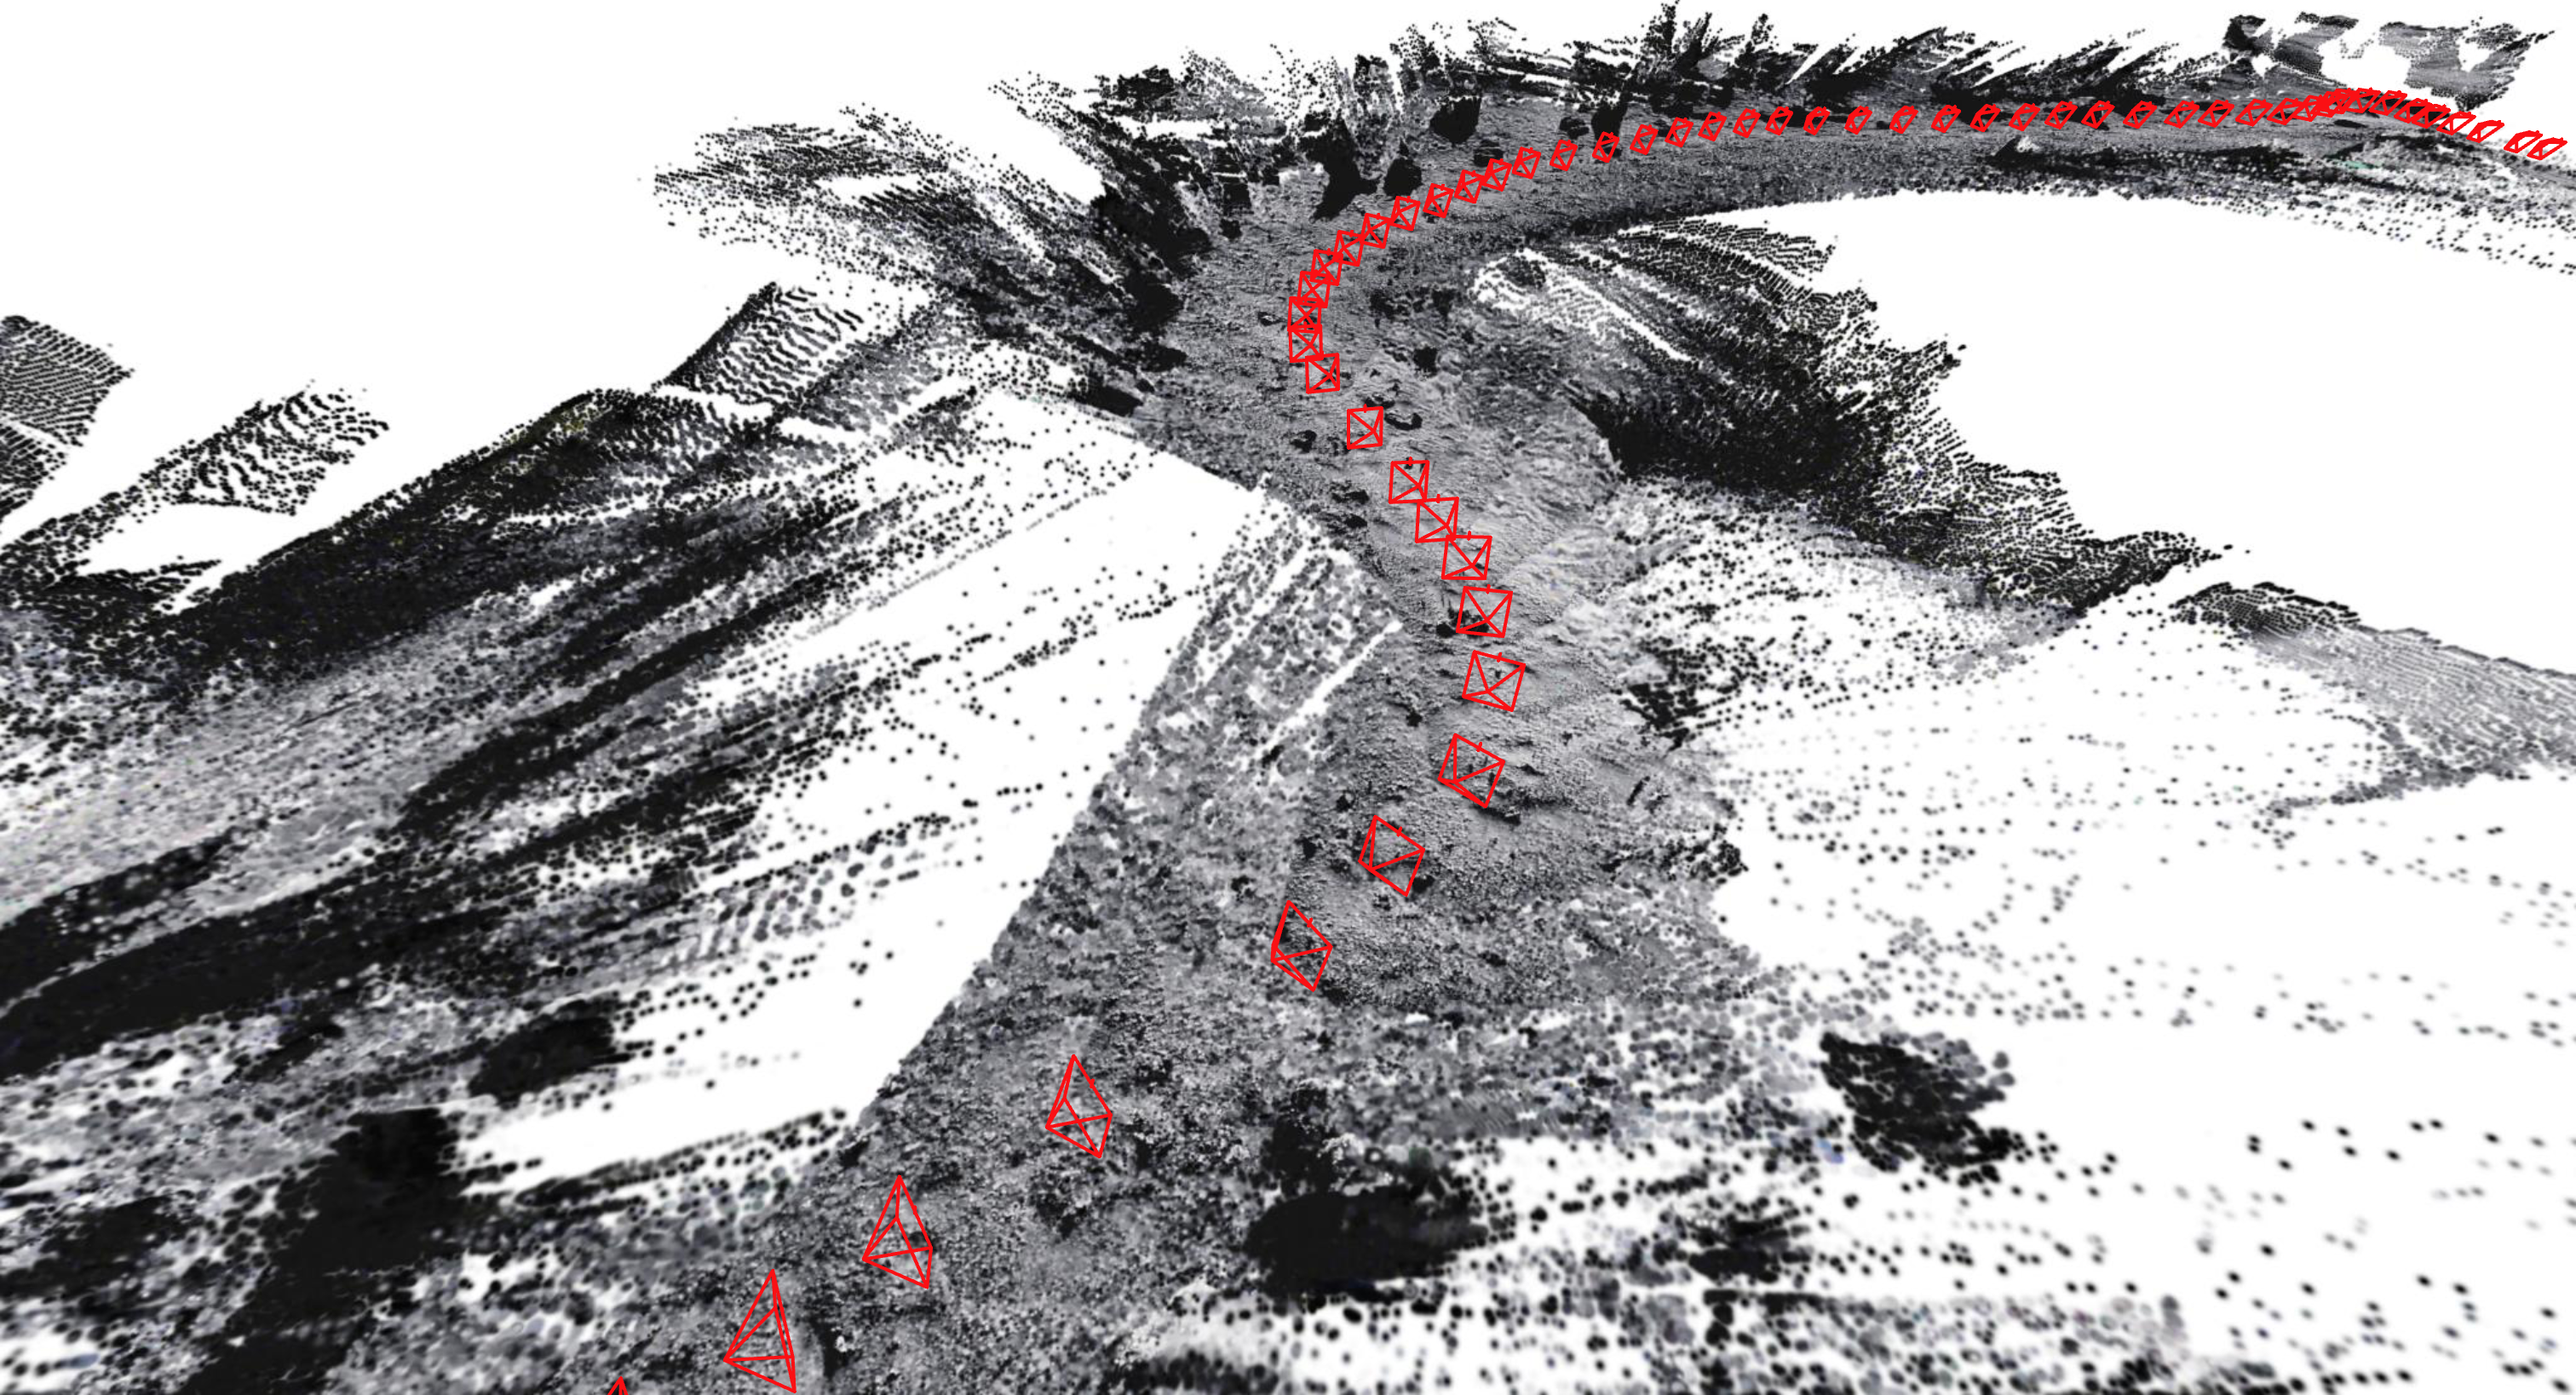
\includegraphics[width=\linewidth]{figures/3dgs/render-2.png}
	\end{subfigure}
	\vspace{1em}
	\begin{subfigure}[b]{0.48\linewidth}
		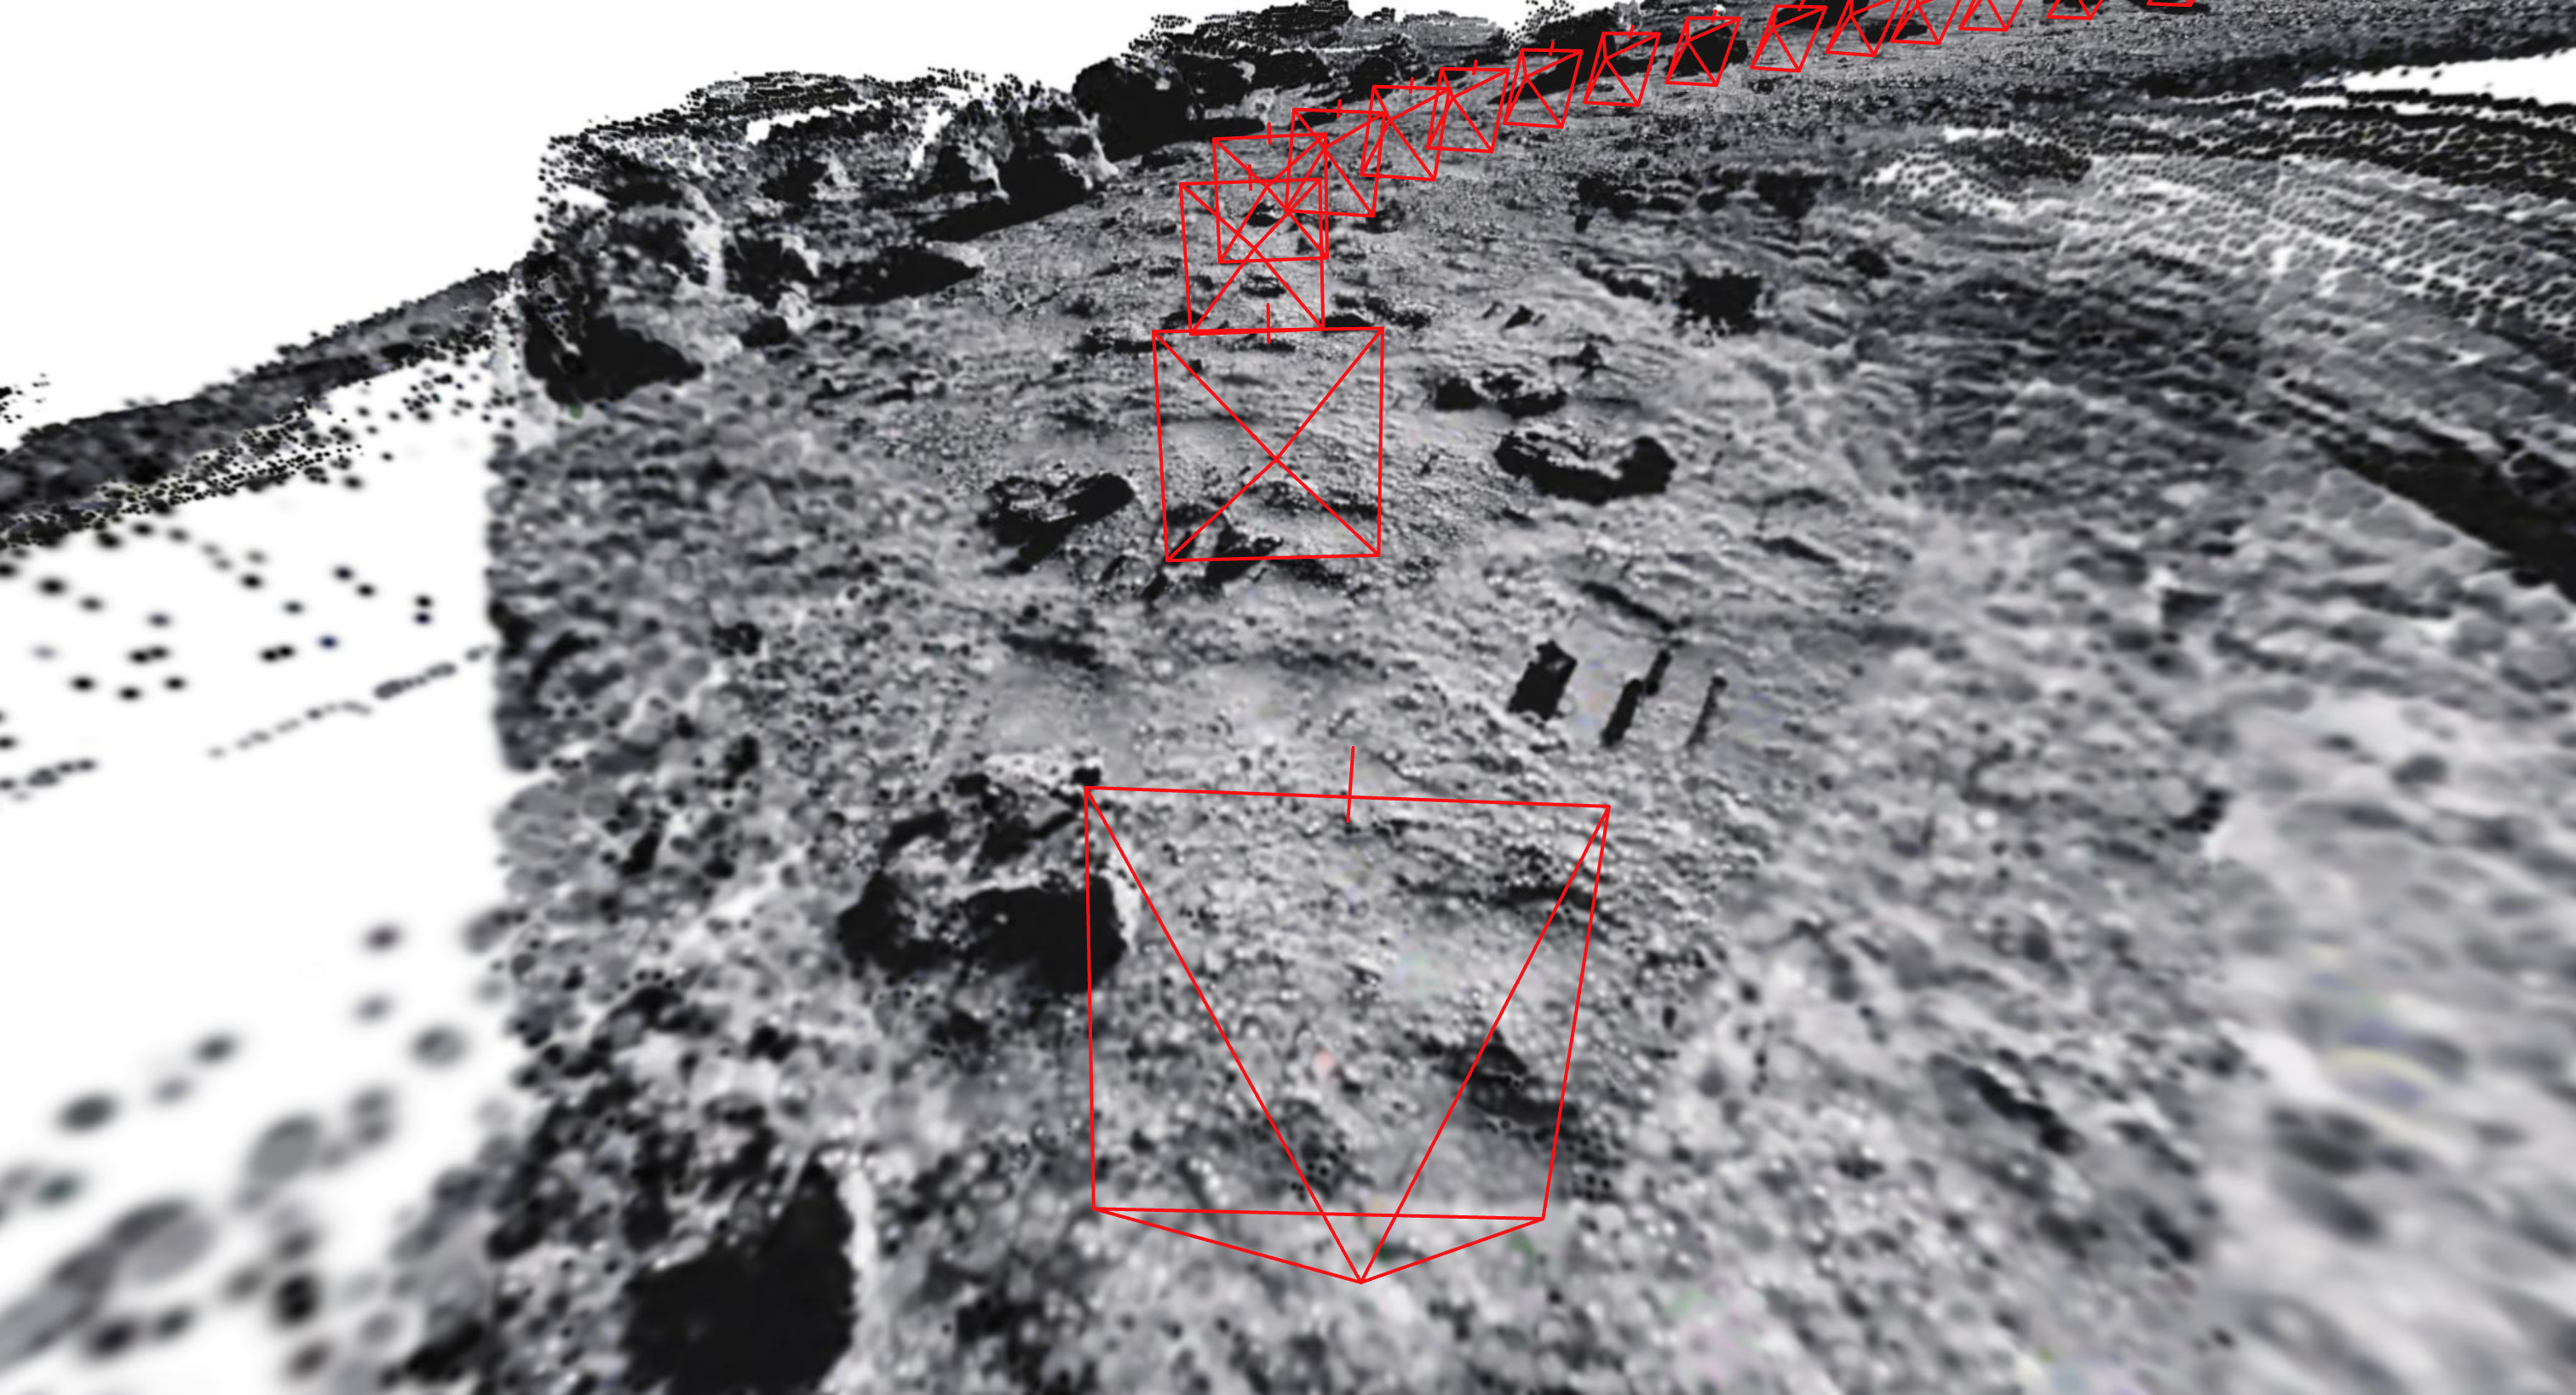
\includegraphics[width=\linewidth]{figures/3dgs/render-3.png}
	\end{subfigure}
	\hfill
	\begin{subfigure}[b]{0.48\linewidth}
		\includegraphics[width=\linewidth]{figures/3dgs/render-4.png}
	\end{subfigure}
	\caption{\bfseries Qualitative results of the real-time 3DGS reconstruction.}
	\label{fig:surface_recon_qual}
\end{figure*}

We implemented our own real-time 3DGS reconstruction pipeline based on Splat-SLAM~\cite{sandstrom_splat-slam_2024} and a point cloud mapping baseline. Our implementation uses ground truth pose information and prior terrain knowledge (without rocks or craters) to initialize the scene. For each new image, we use ground truth segmentation to remove sky regions and tag Gaussians with semantic information, compute depth using our depth estimation models, add new Gaussians to the scene based on RGB and depth information (computing their scale), and optimize the scene in the background using past images. The optimization objective includes L1 RGB and depth losses, penalties for Gaussian density above the surface, Structural Similarity Index Measure (SSIM) loss to ensure the reconstructed images maintain proper structural relationships and perceptual quality compared to the input images, and additional Gaussian regularization terms.
Currently, we do not implement splitting and merging of Gaussians, but we remove Gaussians that are far from the prior terrain.
\Cref{fig:splat-slam} shows the steps of the pipeline using the custom Open3D environment.

\Cref{fig:map_3dgs} shows the 3DGS and point cloud map reconstructions on the Open3D environment, Table~\ref{tab:surface_reconstruction} shows the surface reconstruction and rock detection results, and \cref{fig:novel_views} shows a top view of the 3DGS map. Gaussian splatting with RAFT-Stereo depth outperforms the point cloud baseline in reconstruction accuracy, likely due to its joint optimization over depth and RGB data across multiple views. This demonstrates the potential of neural scene representations for SLAM applications. When ground truth depth is used, the point cloud baseline performs slightly better. We attribute this to our current approach of reconstructing the mesh from the centers of the Gaussians rather than accounting for their density.

In both cases, most errors occur around rocks, which are often dark and hard to distinguish from the sky, making depth estimation challenging. Rock detection performance is comparable between methods, while the point cloud baseline yields lower height error—-possibly due to differences in how the mesh is extracted from the 3DGS map.

\begin{table*}[h]
	\centering
	\small
	\caption{\bfseries Surface reconstruction results. TO BE UPDATED}
	\label{tab:surface_reconstruction}
	\begin{tabular}[t]{|lrrrrrr|}
		\hline
		\multirow{2}{*}{\textbf{Metric}}               &
		\multicolumn{1}{c}{\textbf{Accuracy}}          &
		\multicolumn{1}{c}{\textbf{Completion}}        &
		\multicolumn{1}{c}{\textbf{Precision}}         &
		\multicolumn{1}{c}{\textbf{Recall}}            &
		\multicolumn{1}{c}{\textbf{F-Score}}           &
		\multicolumn{1}{c|}{\textbf{Height Error}}
		\\
		\multicolumn{1}{|c}{}                          &
		\multicolumn{1}{c}{\textbf{[cm] $\downarrow$}} &
		\multicolumn{1}{c}{\textbf{[cm] $\downarrow$}} &
		\multicolumn{1}{c}{\textbf{[\%] $\uparrow$}}   &
		\multicolumn{1}{c}{\textbf{[\%] $\uparrow$}}   &
		\multicolumn{1}{c}{\textbf{[\%] $\uparrow$}}   &
		\multicolumn{1}{c|}{\textbf{[cm] $\downarrow$}}
		\\
		\hline\hline
		\multicolumn{7}{|l|}{\textbf{3DGS}}                                                       \\
		Rock                                           & 61.3  & 27.0 & 13.7 & 26.7 & 18.1 & 15.4 \\
		Regolith                                       & 12.9  & 28.0 & 60.0 & 66.8 & 63.2 & 8.2  \\
		Crater                                         & 941.1 & 27.0 & 9.9  & 15.3 & 12.0 & 74.6 \\
		All                                            & 17.5  & 25.8 & 53.2 & 60.7 & 56.7 & 10.4 \\
		\multicolumn{7}{|l|}{\textbf{ + Ground Truth Depth and Segmentation}}                     \\
		Rock                                           & 61.3  & 27.0 & 13.7 & 26.7 & 18.1 & 15.4 \\
		Regolith                                       & 12.9  & 28.0 & 60.0 & 66.8 & 63.2 & 8.2  \\
		Crater                                         & 941.1 & 27.0 & 9.9  & 15.3 & 12.0 & 74.6 \\
		All                                            & 17.5  & 25.8 & 53.2 & 60.7 & 56.7 & 10.4 \\
		\hline
		\multicolumn{7}{|l|}{\textbf{Point Cloud}}                                                \\
		Rock                                           & 61.3  & 27.0 & 13.7 & 26.7 & 18.1 & 15.4 \\
		Regolith                                       & 12.9  & 28.0 & 60.0 & 66.8 & 63.2 & 8.2  \\
		Crater                                         & 941.1 & 27.0 & 9.9  & 15.3 & 12.0 & 74.6 \\
		All                                            & 17.5  & 25.8 & 53.2 & 60.7 & 56.7 & 10.4 \\
		\multicolumn{7}{|l|}{\textbf{+ Ground Truth Depth and Segmentation}}                      \\
		Rock                                           & 61.3  & 27.0 & 13.7 & 26.7 & 18.1 & 15.4 \\
		Regolith                                       & 12.9  & 28.0 & 60.0 & 66.8 & 63.2 & 8.2  \\
		Crater                                         & 941.1 & 27.0 & 9.9  & 15.3 & 12.0 & 74.6 \\
		All                                            & 17.5  & 25.8 & 53.2 & 60.7 & 56.7 & 10.4 \\
		\hline
	\end{tabular}
\end{table*}



\begin{table}[h]
	\centering
	\small
	\caption{\bfseries Memory usage for 3DGS.}
	\label{tab:memory_usage}
	\begin{minipage}[t]{0.48\linewidth}
		\centering
		\begin{tabular}[t]{|lr|}
			\hline
			\textbf{GPU VRAM} & 1017 MB \\\hline\hline
			\textbf{3DGS}     & 793 MB  \\
			~~Means           & 170 MB  \\
			~~Scales          & 170 MB  \\
			~~Rotations       & 227 MB  \\
			~~Opacities       & 56 MB   \\\hline
			\textbf{Strategy} & 224 MB  \\
			~~Radii           & 56 MB   \\
			~~Labels          & 56 MB   \\
			~~Gradients       & 56 MB   \\
			~~Counts          & 56 MB   \\\hline
		\end{tabular}
	\end{minipage}%
	\begin{minipage}[t]{0.48\linewidth}
		\centering
		\begin{tabular}[t]{|lr|}
			\hline
			\textbf{System RAM} & 1900 MB \\\hline\hline
			~~RGBs              & 1200 MB \\
			~~Depths            & 400 MB  \\
			~~Masks             & 200 MB  \\
			~~Labels            & 100 MB  \\
			\hline
		\end{tabular}
	\end{minipage}
\end{table}
